
\section{\trEnergySurface{}上的\trPeriodicSolution}
\label{sec:energy-periodic-solutions}

$(M,\omega)$ 上\trHamiltonianVectorField%
\begin{equation}\label{eq:XH-xM}
\dot{x}=X_{H}(x),\qquad x\in M
\end{equation}
的\trFlow{} $\varphi^{t}$ 使\trSmooth{}函数 $H$ 在 $M$ 上的诸\trLevelSet{}保持%
不变，即只要 $t$ 有定义，便有 $H\bigl(\varphi^{t}(x)\bigr)=H(x)$。固定这个\trEnergy{}函数的%
一个值——不妨设其为 $E=1$——我们将要求子集
\begin{equation}\label{eq:S-level-one}
S=\bigl\{\,x\in M\ \bigm|\ H(x)=1\,\bigr\}
\end{equation}
是\trCompact{}且\trRegular{}的，即
\begin{equation}\label{eq:dH-nonzero}
dH(x)\neq0\quad\text{对}\quad x\in S.
\end{equation}
于是 $S\subset M$ 是一个\trSmooth{}且\trCompact{}的\trSubmanifold，其%
\trCodimension{}为 $1$，它在点 $x\in S$ 处的\trTangentSpace{}由
\begin{equation}\label{eq:tangent-space-S}
T_{x}S=\bigl\{\,\xi\in T_{x}M\ \bigm|\ dH(x)\xi=0\,\bigr\}.
\end{equation}
给出。由\trHamiltonianVectorField{}的定义可知 $X_{H}(x)\in T_{x}S$，故 $X_{H}$%
是 $S$ 上一个处处非零的\trVectorField；又因 $S$ \trCompact，其\trFlow{}对一切%
时刻都存在。我们的目标便是求出 $X_{H}$ 在\trEnergySurface{} $S$ 上的%
\trPeriodicSolution。这正是引言中所描述的那个定性存在性问题。

为了说明所用的方法，我们先从一个初步结果入手。诀窍在于把给定的%
\trEnergySurface{} $S$ 加厚，并考察一个由能量参数化的单参数曲面族。由于%
$S$ \trCompact{}且\trRegular，故存在 $S$ 的一个开而有界的\trNeighborhood{}%
$U$，它由一些\trEnergy{}值靠近 $E=1$ 的\trCompact{}且\trRegular{}的%
\trEnergySurface{}填满：
\begin{equation}\label{eq:U-union}
U=\bigcup_{\lambda\in I}S_{\lambda},
\end{equation}
其中 $I$ 是绕 $\lambda=1$ 的一个开区间，而%
$S_{\lambda}=\bigl\{\,x\in U\ \bigm|\ H(x)=\lambda\,\bigr\}$ 与给定的\trSurface{}%
$S$ \trDiffeomorphic，后者对应于参数值 $\lambda=1$。的确，在 $M$ 上任取一个%
\trRiemann{}度量，则由 \eqref{eq:dH-nonzero}，%
$H$ 关于此度量的\trGradient{}在 $S$ 的一个\trNeighborhood{}内不消失，即%
$\nabla H\neq0$。于是，我们可以在 $S$ 附近定义修正的\trGradient{}\trVectorField
\[
\dot{x}=\frac{\nabla H(x)}{\lvert\nabla H(x)\rvert^{2}}
\]
它与 $S$ \trTransversal。其\trFlow{} $\psi^{t}$ 满足
\[
H\bigl(\psi^{t}(x)\bigr)=1+t
\]
（$x\in S$），从而定义了一个\trDiffeomorphism{} $(x,t)\mapsto\psi^{t}(x)$，%
它把 $S\times(-\varepsilon,\varepsilon)$ 映满 $S$ 的一个开\trNeighborhood{}%
$U$，正如所断言的。

\begin{theorem}[\trHofer-\trZehnder]\label{thm:hz-energy-surface}
设 $S$ 是 $(M,\omega)$ 上\trHamiltonianVectorField{} $X_{H}$ 的一张%
\trCompact\trRegular\trEnergySurface。假设存在 $S$ 的一个开\trNeighborhood{}%
$U$，其\trCapacity{}有界：$c_{0}(U,\omega)<\infty$。那么，存在一列\trEnergy{}值%
$\lambda_{j}\to1$，使得 $X_{H}$ 在每张\trEnergySurface{} $S_{\lambda_{j}}$ 上都%
有一个\trPeriodicSolution。
\end{theorem}

实际上，这个证明还建立了更多的解：

\begin{corollary}\label{cor:dense-energy-values}
存在\trDense{}子集 $\Sigma\subset I$，使得对 $\lambda\in\Sigma$，只要%
$c_{0}(U,\omega)<\infty$，\trEnergySurface{} $S_{\lambda}$ 便具有 $X_{H}$ 的一个%
\trPeriodicSolution。
\end{corollary}

应当强调，除「一个有界的开\trNeighborhood{}必须具有有限\trCapacity{}」之外，%
对给定的\trRegular{}且\trCompact{}的\trEnergySurface{} $S$ 无需任何其他假设。%
例如，在\trStandard\trSymplecticManifold{} $(\R^{2n},\omega_{0})$ 的特殊情形中，%
有界集 $U$ 含于某个大的\trBall{} $B(R)$ 之中，从而由\trCapacity{}的%
\trMonotonicity，它总具有有限的\trCapacity。于是，$\R^{2n}$ 中每张%
\trCompact\trRegular\trEnergySurface{} $S$ 都会产生大量的\trPeriodicSolution，%
它们属于那些\trEnergy{}靠近给定能量值的\trHamiltonianVectorField{} $X_{H}$。

\begin{proof}
这个论断是特殊\trCapacity{} $c_{0}$ 之定义的直接推论，只要回顾引言中的提示：%
在选取表示诸\trEnergySurface{}的、合乎便利的\trHamiltonianFunction{}时，我们%
享有自由。我们将在 $U$ 上构造一个辅助\trHamiltonianFunction{} $F$，它在含于%
$U$ 内的每张\trSurface{} $S_{\lambda}$ 上取常值，并且此外还属于前一章中所定义%
的函数集 $\mathcal{H}(U,\omega)$。

设 $I=\{\,1-\rho<\lambda<1+\rho\,\}$（$\rho>0$ 为某数），我们选取%
$\varepsilon$ 使 $0<\varepsilon<\rho$。由于按假设 $c_{0}(U,\omega)<\infty$，%
我们可以选取\trSmooth{}函数 $f:\R\to\R$ 满足：
\begin{align*}
f(s)\ &=\ c_{0}(U,\omega)+1 && \text{对}\ s\leq1-\varepsilon\quad\text{及}%
\quad s\geq1+\varepsilon\\
f(s)\ &=\ 0 && \text{对}\ 1-\tfrac{\varepsilon}{2}\leq s\leq1+\tfrac{\varepsilon}{2}\\
f'(s)\ &<\ 0 && \text{对}\ 1-\varepsilon<s<1-\tfrac{\varepsilon}{2}\\
f'(s)\ &>\ 0 && \text{对}\ 1+\tfrac{\varepsilon}{2}<s<1+\varepsilon.
\end{align*}

\noindent\begin{minipage}{\linewidth}
\centering
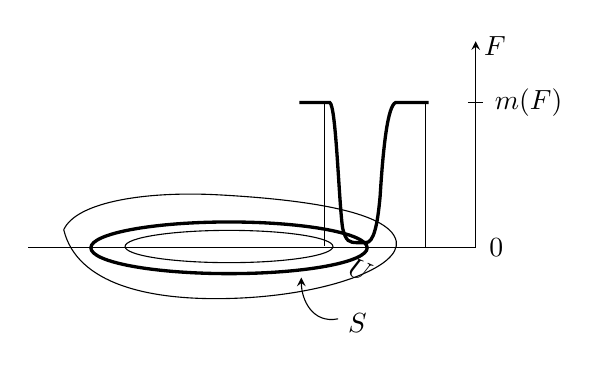
\begin{tikzpicture}[>=stealth,scale=0.82]
  \draw (1.75,0) -- (8.68,0);%
  \draw[->] (8.68,0) -- (8.68,3.2);%
  \node at (8.98,3.12) {$F$};
  \draw (8.56,2.25) -- (8.8,2.25);%
  \node at (9.5,2.25) {$m(F)$};
  \node at (9.0,0) {$0$};
  \draw (2.3,0.28) .. controls (2.5,0.72) and (3.6,0.88) .. (4.7,0.82)
        .. controls (5.8,0.76) and (7.35,0.6) .. (7.45,0.1)
        .. controls (7.52,-0.3) and (6.4,-0.72) .. (5.0,-0.78)
        .. controls (3.6,-0.84) and (2.5,-0.55) .. (2.3,0.28);%
  \draw[very thick] (4.86,0) ellipse (2.14 and 0.4);%
  \draw (4.86,0.02) ellipse (1.61 and 0.25);%
  \node[rotate=-24] at (6.9,-0.35) {$U$};
  \draw[->] (6.55,-1.1) .. controls (6.15,-1.18) and (5.98,-0.8) .. (5.98,-0.46);%
  \node at (6.85,-1.17) {$S$};
  \draw[very thick] (5.95,2.25) -- (6.42,2.25)
        .. controls (6.52,2.2) and (6.56,0.7) .. (6.62,0.3)
        .. controls (6.67,0.1) and (6.72,0.08) .. (6.85,0.08)
        -- (6.98,0.08)
        .. controls (7.1,0.08) and (7.16,0.35) .. (7.2,0.8)
        .. controls (7.25,1.6) and (7.32,2.2) .. (7.44,2.25)
        -- (7.95,2.25);%
  \draw[very thin] (6.33,2.25) -- (6.33,0.03);%
  \draw[very thin] (7.9,2.25) -- (7.9,0);%
\end{tikzpicture}

图 4.1
\end{minipage}

\noindent\begin{minipage}{\linewidth}
\centering
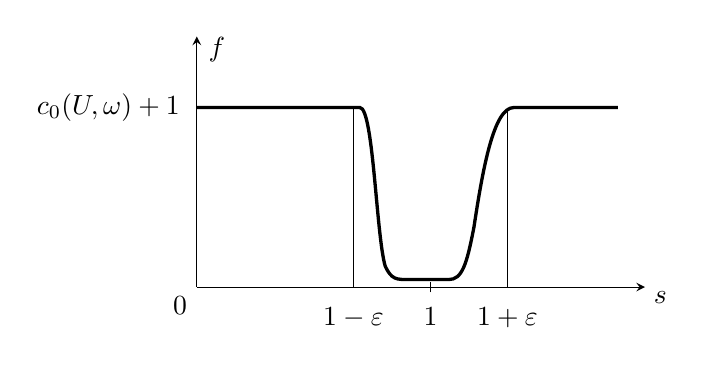
\begin{tikzpicture}[>=stealth,x=1.15cm,y=0.95cm]
  \draw[->] (0,0) -- (0,3.35);%
  \node at (0.22,3.18) {$f$};
  \draw[->] (0,0) -- (4.95,0);%
  \node at (5.12,-0.14) {$s$};
  \node[left] at (-0.08,2.4) {$c_{0}(U,\omega)+1$};
  \draw[very thin] (1.73,2.4) -- (1.73,0);%
  \draw[very thin] (3.43,2.4) -- (3.43,0);%
  \draw[very thick] (0,2.4) -- (1.8,2.4)
        .. controls (1.95,2.4) and (1.98,0.7) .. (2.08,0.28)
        .. controls (2.15,0.1) and (2.2,0.1) .. (2.35,0.1)
        -- (2.78,0.1)
        .. controls (2.93,0.1) and (2.98,0.3) .. (3.06,0.8)
        .. controls (3.16,1.6) and (3.28,2.4) .. (3.5,2.4)
        -- (4.65,2.4);%
  \draw (2.58,-0.07) -- (2.58,0.07);%
  \node[below left] at (0,0) {$0$};
  \node[below] at (1.73,-0.14) {$1-\varepsilon$};
  \node[below] at (2.58,-0.14) {$1$};
  \node[below] at (3.43,-0.14) {$1+\varepsilon$};
\end{tikzpicture}

图 4.2
\end{minipage}

定义 $F:U\to\R$ 如下：
\[
F(x)=f\bigl(H(x)\bigr),\qquad x\in U.
\]
则 $F\in\mathcal{H}(U,\omega)$，且 $m(F)>c_{0}(U,\omega)$。于是，按\trCapacity{}%
$c_{0}(U,\omega)$ 的定义，\trHamiltonianSystem
\[
\dot{x}=X_{F}(x),\qquad x\in U.
\]
拥有一个\trPeriodic{}满足 $0<T\leq1$ 的非常值\trPeriodicSolution{} $x(t)$。

由\trHamiltonianVectorField{}的定义，%
$\omega\bigl(X_{F}(x),\cdot\,\bigr)=-dF(x)=-f'\bigl(H(x)\bigr)dH(x)=%
\omega\bigl(f'\bigl(H(x)\bigr)X_{H}(x),\cdot\,\bigr)$，从而
\[
X_{F}(x)=f'\bigl(H(x)\bigr)\cdot X_{H}(x),\qquad x\in U.
\]
此外，
\[
H\bigl(x(t)\bigr)=\lambda
\]
关于 $t$ 为常数，这是因为%
$\frac{d}{dt}H\bigl(x(t)\bigr)=dH\bigl(x(t)\bigr)\cdot\dot{x}(t)=%
f'(H)\cdot\omega(X_{H},X_{H})=0$。由于 $x(t)$ 不是常值解，我们得出
\[
f'\bigl(H\bigl(x(t)\bigr)\bigr)=f'(\lambda)=\tau\neq0.
\]
于是，按函数 $f$ 的定义，值 $\lambda$ 属于集合%
$1-\varepsilon<\lambda<1-\tfrac{\varepsilon}{2}$ 或%
$1+\tfrac{\varepsilon}{2}<\lambda<1+\varepsilon$。特别地，$|\lambda-1|<\varepsilon$。%
作\trReparametrization，我们定义\trClosed\trCurve{} $y:\R\to S_{\lambda}$
\[
y(t)=x\Bigl(\frac{t}{\tau}\Bigr)
\]
其\trPeriodic{}为 $|\tau|T$\footnote{原书印作「$\tau T$」，未顾及 $\tau=f'(\lambda)$ 在左侧过渡区间 $1-\varepsilon<\lambda<1-\tfrac{\varepsilon}{2}$ 内取负值，重参数化曲线的正周期应为 $|\tau|T$，此处径改。——译者注}，且满足
\[
\dot{y}(t)=\frac{1}{\tau}\dot{x}\Bigl(\frac{t}{\tau}\Bigr)=X_{H}\bigl(y(t)\bigr),
\]
因而是原\trHamiltonianVectorField{} $X_{H}$ 在\trEnergySurface{}%
$H\bigl(y(t)\bigr)=\lambda$ 上的一个\trPeriodicSolution；并且%
$|\lambda-1|<\varepsilon$。由于 $\varepsilon$ 是任意的，定理得证。把 $\lambda=1$%
换成区间 $I$ 中任何其他的 $\lambda$ 值，用同一论证，我们也证明了推论。
\end{proof}

必须记住，\cref{thm:hz-energy-surface} 所保证的诸\trPeriodicSolution{}是非常%
特殊的。它们的确是间接地通过隐藏在\trSymplecticInvariant{} $c_{0}$ 构造中的%
一条特殊\trVariationalPrinciple{}找到的，因而可能还存在许多别的%
\trPeriodicSolution。此外，这些\trPeriodicSolution{}未必位于 $X_{H}$ 的给定%
\trEnergySurface{} $S$ 上，而只是位于其附近。然而，如果我们另外还知道%
$X_{H}$ 在诸 $S_{\lambda_{j}}$ 上的\trPeriodicSolution{} $x_{j}$ 的\trPeriodic{}%
$T_{j}$ 是有界的，便能断定 $S$ 本身也具有\trPeriodicSolution。这一简单的观察%
在下文中会非常有用。确切地说，我们在 $M$ 上选取一个\trRiemann{}度量 $g$，%
并简记 $g(x)(\xi,\eta)=\langle\xi,\eta\rangle$ 与%
$g(x)(\xi,\xi)=\lvert\xi\rvert^{2}$\footnote{原书印作「$g(x)\langle\xi,\xi\rangle=|\xi|^{2}$」，第二处尖括号疑为圆括号之误，此处径改。——译者注}。若 $x(t)$ 是\trPeriodic{}为 $T$ 的%
\trPeriodicSolution，则可引入其长度
\[
l(x)=\int_{0}^{T}\ \lvert\dot{x}(t)\rvert\,dt.
\]
必要时收缩开\trNeighborhood{} $U$ 之后，我们可以假设
\[
C^{-1}\ \leq\ \lvert X_{H}(x)\rvert\ \leq\ C,\qquad x\in U
\]
对某常数 $C>0$ 成立。由于诸 $x_{j}(t)$ 求解\trHamiltonianEquation{}%
$\dot{x}_{j}(t)=X_{H}\bigl(x_{j}(t)\bigr)$，我们得出
\[
C^{-1}\cdot T_{j}\ \leq\ l(x_{j})\ \leq\ C\cdot T_{j}.
\]

\begin{proposition}\label{prop:bounded-periods-limit}
设 $\lambda_{j}\to1$，并假设 $S_{\lambda_{j}}$ 上诸\trPeriodicSolution{}%
$x_{j}(t)$ 的\trPeriodic{} $T_{j}$（或等价地，其长度 $l(x_{j})$）有界。那么%
$S=S_{1}$ 具有 $X_{H}$ 的一个\trPeriodicSolution。
\end{proposition}
\begin{proof}
把诸\trPeriodic{}规范到 $1$，我们定义 $y_{j}(t)=x_{j}(T_{j}\cdot t)$（%
$0\leq t\leq1$），于是
\[
\dot{y}_{j}(t)=T_{j}X_{H}\bigl(y_{j}(t)\bigr)
\]
且 $H\bigl(y_{j}(t)\bigr)=\lambda_{j}$。由于右端按假设是有界的，借助%
\trArzela-\trAscoli{}定理可以找到一个子序列，使得 $T_{j}\to T$、$y_{j}\to y$，%
其收敛起初在 $C^{0}$ 中，继而利用方程，在 $C^{\infty}$ 中也成立。函数%
$y:[0,1]\to U$ 是\trPeriodic{}为 $1$ 的周期函数，满足 $H\bigl(y(t)\bigr)=1$，%
并且
\[
\dot{y}(t)=TX_{H}\bigl(y(t)\bigr),
\]
故当 $T\neq0$ 时它就是所要的\trPeriodicSolution。用反证法，设 $T=0$。则%
$y_{j}\to\{y^{*}\}$ 收缩为一点 $y^{*}$，且%
$X_{H}\bigl(y_{j}(t)\bigr)\to X_{H}(y^{*})=V$。由于\trEnergySurface{} $S$ 是%
\trRegular{}的，$V\neq0$。在点 $y^{*}$ 附近的局部坐标中，我们可以估计
\[
\bigl\langle X_{H}(y_{j}),V\bigr\rangle\ \geq\ (1-\varepsilon)\,\lvert V\rvert^{2}
\]
对某个小的 $\varepsilon>0$ 与一切充分大的 $j$ 成立，于是
\[
T_{j}^{-1}\,\bigl\langle\dot{y}_{j}(t),V\bigr\rangle\ \geq\ (1-\varepsilon)\,%
\lvert V\rvert^{2}.
\]
沿一个\trPeriodic{}积分，我们得出 $V=0$，与 $V\neq0$ 矛盾，命题得证。
\end{proof}

在建立了\trHamiltonianVectorField{} $X_{H}$ 之\trPeriodicSolution{}的存在性%
之后，值得记住的是：一般而言，一个\trPeriodicSolution{}属于一个由能量%
参数化的完整的\trPeriodicSolution{}族。这一点将由所谓的\trPoincare{}%
\trContinuation{}方法来证明。这一局部技巧以\trImplicitFunctionTheorem{}为%
基础，并且需要对给定\textbf{\trReferenceSolution}（reference solution）的\trFloquet{}乘子有所了解。

考察 $X_{H}$ 的一个\trPeriodicSolution{} $x(t)=x(t,E^{*})$，其\trEnergy{}为%
$E^{*}=H\bigl(x(t)\bigr)$，\trPeriodic{}为 $T=T^{*}$。由于\trVectorField{}%
$X_{H}$ 不依赖时间，$x(t)$ 的诸\trFloquet{}乘子中必有一个等于 $1$。的确，%
简记 $x=x(0)$，把\trFlow{}的等式%
$\varphi^{t}\circ\varphi^{s}(x)=\varphi^{s}\circ\varphi^{t}(x)$ 在 $s=0$ 处对%
$s$ 求导，便得到
\[
d\varphi^{t}(x)X_{H}(x)=X_{H}\bigl(\varphi^{t}(x)\bigr)
\]
对一切 $t$ 成立。若 $t=T$ 是\trPeriodic，从而 $\varphi^{T}(x)=x$，则得到
\[
d\varphi^{T}(x)X_{H}(x)=X_{H}(x)\ \in\ T_{x}M.
\]
按定义，\trLinear{}映射 $d\varphi^{T}(x):T_{x}M\to T_{x}M$ 的诸\trEigenvalue{}%
就是\trPeriodicSolution{} $x(t)$ 的诸\trFloquet{}乘子，而我们刚刚验证了 $1$%
总是一个\trFloquet{}乘子。但由于 $d\varphi^{T}(x)$ 是\trSymplectic\trLinear{}%
映射，\trEigenvalue{} $1$ 必具有偶\trMultiplicity，故 $x(t)$ 总具有至少两个%
等于 $1$ 的\trFloquet{}乘子。实际上，我们将在下述命题的证明过程中验证这一点；%
该命题早已为 H.~\trPoincare{}所知。

\begin{proposition}\label{prop:poincare-continuation}
设 $X_{H}$ 在 $M$ 上有一个\trPeriodicSolution{} $x(t,E^{*})$，其\trEnergy{}%
$E^{*}=H\bigl(x(t,E^{*})\bigr)$、\trPeriodic{}为 $T^{*}$，并且恰有两个%
\trFloquet{}乘子等于 $1$。那么，存在唯一而\trSmooth{}的\trPeriodicSolution{}%
单参数族 $x(t,E)$，其诸\trPeriodic{} $T(E)$ 靠近 $T^{*}$，并且位于诸%
\trEnergySurface
\[
H\bigl(x(t,E)\bigr)=E
\]
之上，这里 $\lvert E-E^{*}\rvert$ 充分小。此外，当 $E\to E^{*}$ 时%
$T(E)\to T(E^{*})$。
\end{proposition}

暂且把证明搁置一旁，我们注意到：\trReferenceSolution{} $x(t,E^{*})$ 作为\trPeriodicSolution{}%
在 $M$ 中并不是孤立的。诸\trPeriodicSolution{} $x(t,E)$ 对应于不同的 $E$ 值，%
而且在证明中将看到：在固定的\trEnergySurface{} $E$ 上，这个解在那些%
\trPeriodic{}靠近 $T$ 的\trPeriodicSolution{}之中是孤立的。从几何上看，诸%
\trPeriodicSolution{} $x(t,E)$ 在 $M$ 中填满一个\trEmbedding{}的\trCylinder，%
正如下图 4.3 所描绘的那样。

\noindent\begin{minipage}{\linewidth}
\centering
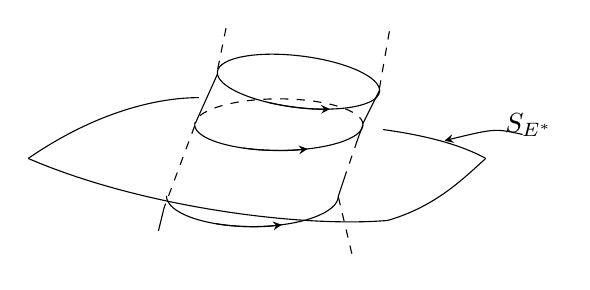
\begin{tikzpicture}[>=stealth,scale=0.78]
  \begin{scope}[rotate around={-7:(5.6,2.98)}]
    \draw (5.6,2.98) ellipse (1.33 and 0.42);%
    \draw[->] ([shift={(5.6,2.98)}]250:1.33 and 0.42)
          arc[start angle=250,end angle=295,x radius=1.33,y radius=0.42];%
  \end{scope}
  \draw[dashed] (4.42,3.85) -- (4.28,3.16);%
  \draw[dashed] (7.08,3.8) -- (6.92,2.88);%
  \draw (4.28,3.1) -- (3.92,2.3);%
  \draw (6.92,2.84) -- (6.65,2.3);%
  \draw[dashed] (3.91,2.26) -- (3.41,0.92);%
  \draw (3.41,0.92) -- (3.32,0.55);%
  \draw (6.65,2.28) -- (6.56,2.03);%
  \draw[dashed] (6.56,2.03) -- (6.36,1.45);%
  \draw (6.36,1.45) -- (6.25,1.12);%
  \draw[dashed] (6.25,1.1) -- (6.5,0.05);%
  \draw[dashed] ([shift={(5.28,2.28)}]0:1.37 and 0.42)
        arc[start angle=0,end angle=180,x radius=1.37,y radius=0.42];
  \draw ([shift={(5.28,2.28)}]180:1.37 and 0.42)
        arc[start angle=180,end angle=360,x radius=1.37,y radius=0.42];
  \draw[->] ([shift={(5.28,2.28)}]245:1.37 and 0.42)
        arc[start angle=245,end angle=290,x radius=1.37,y radius=0.42];
  \draw ([shift={(4.85,1.12)}]180:1.4 and 0.5)
        arc[start angle=180,end angle=360,x radius=1.4,y radius=0.5];
  \draw[->] ([shift={(4.85,1.12)}]245:1.4 and 0.5)
        arc[start angle=245,end angle=290,x radius=1.4,y radius=0.5];
  \draw (1.2,1.73) .. controls (2.2,2.42) and (3.2,2.72) .. (3.98,2.72);%
  \draw (6.98,2.2) .. controls (7.7,2.1) and (8.25,1.95) .. (8.65,1.73);%
  \draw (1.2,1.73) .. controls (3.0,0.95) and (5.6,0.6) .. (7.05,0.72)
        .. controls (7.85,0.95) and (8.3,1.42) .. (8.65,1.73);%
  \node at (9.35,2.28) {$S_{E^{*}}$};
  \draw[->] (9.25,2.12) .. controls (8.8,2.22) .. (7.98,2.02);%
\end{tikzpicture}

图 4.3
\end{minipage}

\begin{proof}[\cref*{prop:poincare-continuation}的证明]
回顾一下属于某个\trPeriodicSolution{}的\trTransversalSection\trMapping{}%
之构造，是有益的。设 $x(t)$ 是 $M$ 上某个\trVectorField{} $X$ 的非常值%
\trPeriodicSolution，并以其\trPeriodic{}为 $T>0$。于是，我们可以在点%
$p=x(0)$ 处把 $x(t)$ 与一张 $(2n-1)$ 维的\trHypersurface——即一个满足%
$\operatorname{codim}\Sigma=1$ 的局部\trSubmanifold{} $\Sigma\subset M$——%
相交，使\trVectorField{} $X$ 在其上处处不相切。这意味着，对 $p$ 附近的每个%
$x\in\Sigma$，$T_{x}\Sigma$ 与 $X(x)$ 张成\trTangentSpace{} $T_{x}M$：
\[
T_{x}M=T_{x}\Sigma\oplus\bigl\langle X(x)\bigr\rangle,\qquad x\in\Sigma.
\]

若 $\varphi^{t}$ 表示 $X$ 的\trFlow，则 $\varphi^{T}(p)=p\in\Sigma$。由于%
\trFlow{}对 $x$ 可微地依赖，我们可以在 $p$ 附近局部地定义一个\trSmooth{}映射%
$\psi:\Sigma\to\Sigma$：把初始点 $x\in\Sigma$ 沿着它的解 $\varphi^{t}(x)$ 前进，%
直到再次遇见 $\Sigma$，即
\[
\psi(x)=\varphi^{\tau(x)}(x),\qquad x\in\Sigma.
\]
这里 $\tau=\tau(x)$ 靠近 $T>0$，并且由条件 $\varphi^{\tau}(x)\in\Sigma$ 唯一%
确定。显然 $\psi(p)=p$。映射 $\psi$ 称为\trPeriodicSolution{} $x(t)$ 的%
\trPoincare{}截面映射。对我们来说，重要的是知道\trLinearization{}映射
\[
d\psi(p)\ :\ T_{p}\Sigma\to T_{p}\Sigma
\]
在\trFixedPoint{} $p\in\Sigma$ 处的诸\trEigenvalue。它们与 $x(t)$ 的诸%
\trFloquet{}乘子——即 $d\varphi^{T}(p)$
\[
d\varphi^{T}(p)\ :\ T_{p}M\to T_{p}M
\]
的诸\trEigenvalue{}——之间的关系，由下述引理给出。

\begin{lemma}\label{lem:floquet-section-determinant}
$d\varphi^{T}(p)$ 以 $1$ 为一个\trEigenvalue{}且以 $X(p)$ 为相应的\trEigenvector，%
而其余的\trEigenvalue{}就是 $d\psi(p)$ 的诸\trEigenvalue；也就是说，二者的%
\trCharacteristicPolynomial{}由下式相联系：
\[
\det\bigl(\lambda-d\varphi^{T}(p)\bigr)=(\lambda-1)\det\bigl(\lambda-d\psi(p)\bigr).
\]
\end{lemma}
\begin{proof}
引理的第一部分我们已在上面验证过。在 $p$ 处微分 $\psi$，对%
$\xi\in T_{p}\Sigma$ 我们得到
\begin{align*}
d\psi(p)\xi\ &=\ d\varphi^{T}(p)\xi+\frac{d}{dt}\varphi^{t}\Big|_{t=T}\cdot d\tau(p)\xi\\
&=\ d\varphi^{T}(p)\xi-\lambda(\xi)X(p),
\end{align*}
其中我们已把线性形式 $d\tau(p)\xi$ 简记为 $-\lambda(\xi)$。相对于分解%
$T_{p}M=\langle X(p)\rangle\oplus T_{p}\Sigma$，线性映射 $d\varphi^{T}(p)$%
遂具有表示
\[
d\varphi^{T}(p)=\ \left(\begin{array}{c|c}
1 & \lambda\\
\hline
0 & d\psi(p)
\end{array}\right),
\]
引理便随之立得。
\end{proof}

显然，$\psi$ 在 $p$ 附近的诸\trFixedPoint{}，正是诸\trReferenceSolution{} $x(t)$ 附近那些%
\trPeriodic{}靠近 $T$ 的\trPeriodicSolution{}的初始条件。我们将利用这一观察来%
证明\cref{prop:poincare-continuation}。设 $x(t)$ 是该命题的\trPeriodicSolution。%
则 $H\bigl(x(t)\bigr)=E^{*}$，且在 $x(t)$ 附近 $dH(x)\neq0$；此外%
$dH(X_{H})=0$。于是，我们可以在 $p=x(0)$ 附近引入便利的局部坐标%
$(x_{1},\dots,x_{2n})\in\R^{2n}$，使得 $p$ 对应于 $x^{*}=(E^{*},0,\dots,0)$，%
使得 $H(x_{1},\dots,x_{2n})=x_{1}$，并且进而使 $x_{2n}=0$ 成为一张局部的%
\trTransversalSection{} $\Sigma$。鉴于 $H\bigl(\varphi^{t}(x)\bigr)=H(x)$，%
截面映射 $\psi$ 在这些坐标下表示为
\[
\psi\ :\ \left(\begin{array}{c} x'\\ x'' \end{array}\right)
\longrightarrow\left(\begin{array}{c} \psi'(x',x'')=x'\\ \psi''(x',x'') \end{array}\right).
\]
其中坐标 $(x',x'')\in\Sigma$ 表示 $x'=x_{1}$ 与 $x''=(x_{2},\dots,x_{2n-1})$。%
目标在于求出 $\psi$ 在 $x^{*}$ 附近的诸\trFixedPoint。为此我们只须求解方程
\[
\psi''(x',x'')=x'',
\]
因为第一个方程 $\psi'(x',x'')=x'$ 自动满足。由于按假设 $x^{*}$ 是\trReferenceSolution{}所对应的%
\trFixedPoint，即 $\psi(x^{*})=x^{*}$\footnote{原书印作「Since, by assumption, $\psi(x^{*})=x^{*}$ is a reference solution」，将不动点等式径称作参考解，措辞失当，此处按文义改写。——译者注}，我们可以应用\trImplicitFunctionTheorem，注意到在我们的坐标下，%
线性化映射表示为
\[
d\psi(x^{*})=\ \left(\begin{array}{c|c}
1 & 0\\
\hline
* & \dfrac{\partial}{\partial x''}\psi''(x^{*})
\end{array}\right).
\]
回顾\cref{prop:poincare-continuation}与\cref{lem:floquet-section-determinant}%
的假设，矩阵
\[
\frac{\partial}{\partial x''}\psi''(x^{*})-\mathbf{1}_{2n-2}
\]
是\trNonsingular{}的。因此，存在唯一的映射 $x'\mapsto x''=a(x')$ 求解方程%
$\psi''\bigl(x',a(x')\bigr)=a(x')$。于是，$x'=E$ 与 $x''=a(E)$ 便是满足%
\cref{prop:poincare-continuation}的那些所需\trPeriodicSolution{}在 $\Sigma$ 上的%
初始条件。
\end{proof}

人们很想把\cref{prop:poincare-continuation}应用于由%
\cref{thm:hz-energy-surface} 所保证的诸 $S_{\lambda_{j}}$ 上的%
\trPeriodicSolution，以便当 $\lambda_{j}\to1$\footnote{原书印作「$\lambda_{j}\to 0$」，疑为「$\lambda_{j}\to 1$」之误，此处径改。——译者注} 时在给定的\trEnergySurface{}%
$S$ 上建立\trPeriodicSolution{}的存在性。但遗憾的是，关于这些解的%
\trFloquet{}乘子什么也说不出来。此外，\cref{prop:poincare-continuation}%
本质上是局部性的：整体地看，由\trPeriodicSolution{}构成的\trCylinder{}最终%
可能会与某张\trEnergySurface{}相切。这一情形已由 C.~\trRobinson{}在文献%
[183]（1970 年）中研究过。
